\documentclass[1p]{elsarticle_modified}
%\bibliographystyle{elsarticle-num}

%\usepackage[colorlinks]{hyperref}
%\usepackage{abbrmath_seonhwa} %\Abb, \Ascr, \Acal ,\Abf, \Afrak
\usepackage{amsfonts}
\usepackage{amssymb}
\usepackage{amsmath}
\usepackage{amsthm}
\usepackage{scalefnt}
\usepackage{amsbsy}
\usepackage{kotex}
\usepackage{caption}
\usepackage{subfig}
\usepackage{color}
\usepackage{graphicx}
\usepackage{xcolor} %% white, black, red, green, blue, cyan, magenta, yellow
\usepackage{float}
\usepackage{setspace}
\usepackage{hyperref}

\usepackage{tikz}
\usetikzlibrary{arrows}

\usepackage{multirow}
\usepackage{array} % fixed length table
\usepackage{hhline}

%%%%%%%%%%%%%%%%%%%%%
\makeatletter
\renewcommand*\env@matrix[1][\arraystretch]{%
	\edef\arraystretch{#1}%
	\hskip -\arraycolsep
	\let\@ifnextchar\new@ifnextchar
	\array{*\c@MaxMatrixCols c}}
\makeatother %https://tex.stackexchange.com/questions/14071/how-can-i-increase-the-line-spacing-in-a-matrix
%%%%%%%%%%%%%%%

\usepackage[normalem]{ulem}

\newcommand{\msout}[1]{\ifmmode\text{\sout{\ensuremath{#1}}}\else\sout{#1}\fi}
%SOURCE: \msout is \stkout macro in https://tex.stackexchange.com/questions/20609/strikeout-in-math-mode

\newcommand{\cancel}[1]{
	\ifmmode
	{\color{red}\msout{#1}}
	\else
	{\color{red}\sout{#1}}
	\fi
}

\newcommand{\add}[1]{
	{\color{blue}\uwave{#1}}
}

\newcommand{\replace}[2]{
	\ifmmode
	{\color{red}\msout{#1}}{\color{blue}\uwave{#2}}
	\else
	{\color{red}\sout{#1}}{\color{blue}\uwave{#2}}
	\fi
}

\newcommand{\Sol}{\mathcal{S}} %segment
\newcommand{\D}{D} %diagram
\newcommand{\A}{\mathcal{A}} %arc


%%%%%%%%%%%%%%%%%%%%%%%%%%%%%5 test

\def\sl{\operatorname{\textup{SL}}(2,\Cbb)}
\def\psl{\operatorname{\textup{PSL}}(2,\Cbb)}
\def\quan{\mkern 1mu \triangleright \mkern 1mu}

\theoremstyle{definition}
\newtheorem{thm}{Theorem}[section]
\newtheorem{prop}[thm]{Proposition}
\newtheorem{lem}[thm]{Lemma}
\newtheorem{ques}[thm]{Question}
\newtheorem{cor}[thm]{Corollary}
\newtheorem{defn}[thm]{Definition}
\newtheorem{exam}[thm]{Example}
\newtheorem{rmk}[thm]{Remark}
\newtheorem{alg}[thm]{Algorithm}

\newcommand{\I}{\sqrt{-1}}
\begin{document}

%\begin{frontmatter}
%
%\title{Boundary parabolic representations of knots up to 8 crossings}
%
%%% Group authors per affiliation:
%\author{Yunhi Cho} 
%\address{Department of Mathematics, University of Seoul, Seoul, Korea}
%\ead{yhcho@uos.ac.kr}
%
%
%\author{Seonhwa Kim} %\fnref{s_kim}}
%\address{Center for Geometry and Physics, Institute for Basic Science, Pohang, 37673, Korea}
%\ead{ryeona17@ibs.re.kr}
%
%\author{Hyuk Kim}
%\address{Department of Mathematical Sciences, Seoul National University, Seoul 08826, Korea}
%\ead{hyukkim@snu.ac.kr}
%
%\author{Seokbeom Yoon}
%\address{Department of Mathematical Sciences, Seoul National University, Seoul, 08826,  Korea}
%\ead{sbyoon15@snu.ac.kr}
%
%\begin{abstract}
%We find all boundary parabolic representation of knots up to 8 crossings.
%
%\end{abstract}
%\begin{keyword}
%    \MSC[2010] 57M25 
%\end{keyword}
%
%\end{frontmatter}

%\linenumbers
%\tableofcontents
%
\newcommand\colored[1]{\textcolor{white}{\rule[-0.35ex]{0.8em}{1.4ex}}\kern-0.8em\color{red} #1}%
%\newcommand\colored[1]{\textcolor{white}{ #1}\kern-2.17ex	\textcolor{white}{ #1}\kern-1.81ex	\textcolor{white}{ #1}\kern-2.15ex\color{red}#1	}

{\Large $\underline{12a_{0779}~(K12a_{0779})}$}

\setlength{\tabcolsep}{10pt}
\renewcommand{\arraystretch}{1.6}
\vspace{1cm}\begin{tabular}{m{100pt}>{\centering\arraybackslash}m{274pt}}
\multirow{5}{120pt}{
	\centering
	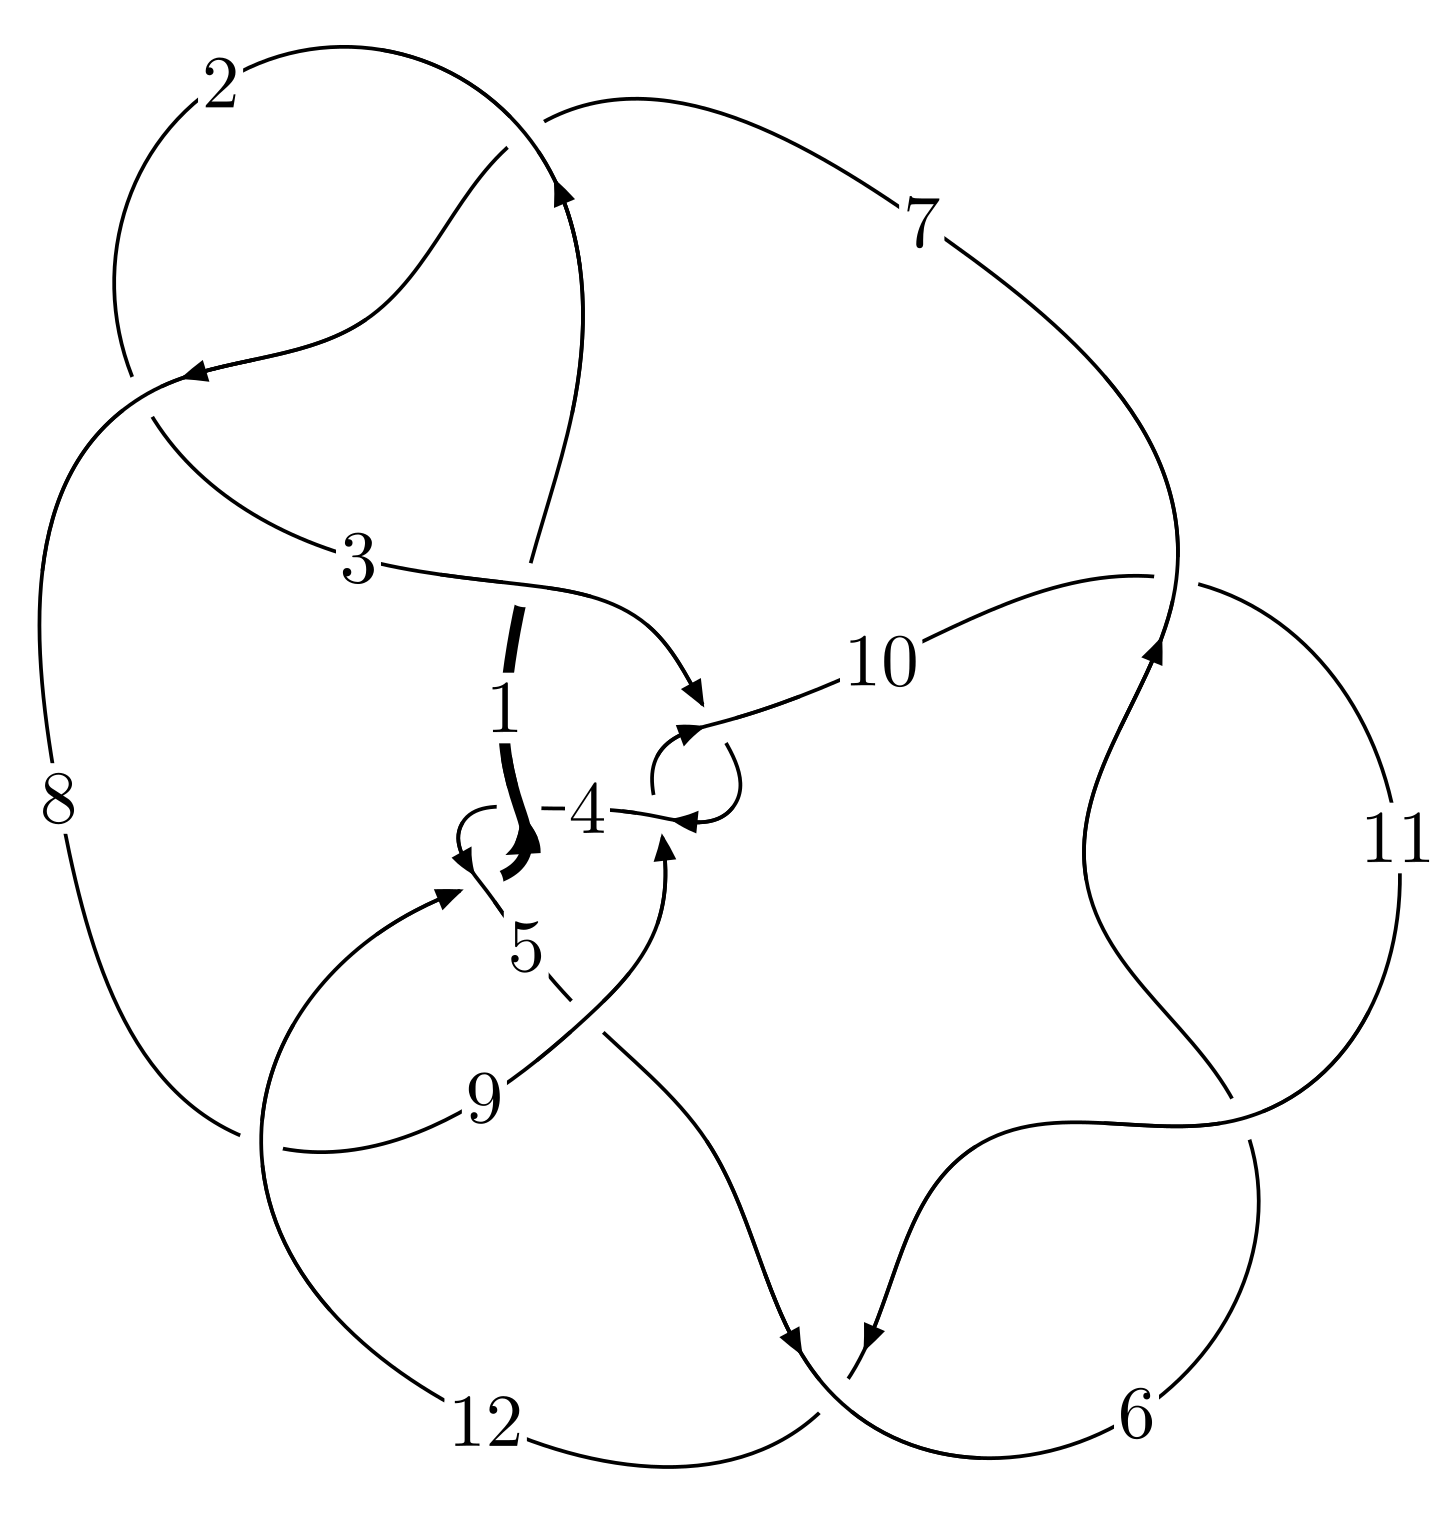
\includegraphics[width=112pt]{../../../GIT/diagram.site/Diagrams/png/1580_12a_0779.png}\\
\ \ \ A knot diagram\footnotemark}&
\allowdisplaybreaks
\textbf{Linearized knot diagam} \\
\cline{2-2}
 &
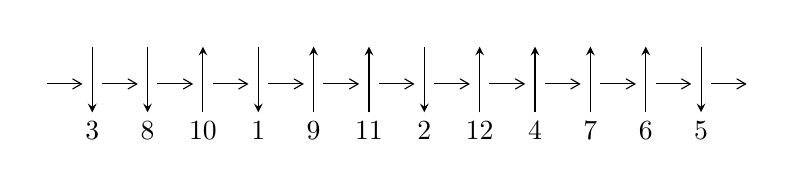
\begin{tikzpicture}[x=20pt, y=17pt]
	% nodes
	\node (C0) at (0, 0) {};
	\node (C1) at (1, 0) {};
	\node (C1U) at (1, +1) {};
	\node (C1D) at (1, -1) {3};

	\node (C2) at (2, 0) {};
	\node (C2U) at (2, +1) {};
	\node (C2D) at (2, -1) {8};

	\node (C3) at (3, 0) {};
	\node (C3U) at (3, +1) {};
	\node (C3D) at (3, -1) {10};

	\node (C4) at (4, 0) {};
	\node (C4U) at (4, +1) {};
	\node (C4D) at (4, -1) {1};

	\node (C5) at (5, 0) {};
	\node (C5U) at (5, +1) {};
	\node (C5D) at (5, -1) {9};

	\node (C6) at (6, 0) {};
	\node (C6U) at (6, +1) {};
	\node (C6D) at (6, -1) {11};

	\node (C7) at (7, 0) {};
	\node (C7U) at (7, +1) {};
	\node (C7D) at (7, -1) {2};

	\node (C8) at (8, 0) {};
	\node (C8U) at (8, +1) {};
	\node (C8D) at (8, -1) {12};

	\node (C9) at (9, 0) {};
	\node (C9U) at (9, +1) {};
	\node (C9D) at (9, -1) {4};

	\node (C10) at (10, 0) {};
	\node (C10U) at (10, +1) {};
	\node (C10D) at (10, -1) {7};

	\node (C11) at (11, 0) {};
	\node (C11U) at (11, +1) {};
	\node (C11D) at (11, -1) {6};

	\node (C12) at (12, 0) {};
	\node (C12U) at (12, +1) {};
	\node (C12D) at (12, -1) {5};
	\node (C13) at (13, 0) {};

	% arrows
	\draw[->,>={angle 60}]
	(C0) edge (C1) (C1) edge (C2) (C2) edge (C3) (C3) edge (C4) (C4) edge (C5) (C5) edge (C6) (C6) edge (C7) (C7) edge (C8) (C8) edge (C9) (C9) edge (C10) (C10) edge (C11) (C11) edge (C12) (C12) edge (C13) ;	\draw[->,>=stealth]
	(C1U) edge (C1D) (C2U) edge (C2D) (C3D) edge (C3U) (C4U) edge (C4D) (C5D) edge (C5U) (C6D) edge (C6U) (C7U) edge (C7D) (C8D) edge (C8U) (C9D) edge (C9U) (C10D) edge (C10U) (C11D) edge (C11U) (C12U) edge (C12D) ;
	\end{tikzpicture} \\
\hhline{~~} \\& 
\textbf{Solving Sequence} \\ \cline{2-2} 
 &
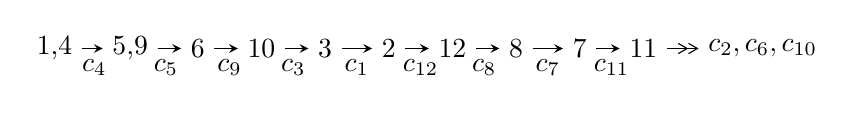
\begin{tikzpicture}[x=23pt, y=7pt]
	% node
	\node (A0) at (-1/8, 0) {1,4};
	\node (A1) at (17/16, 0) {5,9};
	\node (A2) at (17/8, 0) {6};
	\node (A3) at (25/8, 0) {10};
	\node (A4) at (33/8, 0) {3};
	\node (A5) at (41/8, 0) {2};
	\node (A6) at (49/8, 0) {12};
	\node (A7) at (57/8, 0) {8};
	\node (A8) at (65/8, 0) {7};
	\node (A9) at (73/8, 0) {11};
	\node (C1) at (1/2, -1) {$c_{4}$};
	\node (C2) at (13/8, -1) {$c_{5}$};
	\node (C3) at (21/8, -1) {$c_{9}$};
	\node (C4) at (29/8, -1) {$c_{3}$};
	\node (C5) at (37/8, -1) {$c_{1}$};
	\node (C6) at (45/8, -1) {$c_{12}$};
	\node (C7) at (53/8, -1) {$c_{8}$};
	\node (C8) at (61/8, -1) {$c_{7}$};
	\node (C9) at (69/8, -1) {$c_{11}$};
	\node (A10) at (11, 0) {$c_{2},c_{6},c_{10}$};

	% edge
	\draw[->,>=stealth]	
	(A0) edge (A1) (A1) edge (A2) (A2) edge (A3) (A3) edge (A4) (A4) edge (A5) (A5) edge (A6) (A6) edge (A7) (A7) edge (A8) (A8) edge (A9) ;
	\draw[->>,>={angle 60}]	
	(A9) edge (A10);
\end{tikzpicture} \\ 

\end{tabular} \\

\footnotetext{
The image of knot diagram is generated by the software ``\textbf{Draw programme}" developed by Andrew Bartholomew(\url{http://www.layer8.co.uk/maths/draw/index.htm\#Running-draw}), where we modified some parts for our purpose(\url{https://github.com/CATsTAILs/LinksPainter}).
}\phantom \\ \newline 
\centering \textbf{Ideals for irreducible components\footnotemark of $X_{\text{par}}$} 
 
\begin{align*}
I^u_{1}&=\langle 
6.88485\times10^{431} u^{115}-3.87633\times10^{432} u^{114}+\cdots+3.06291\times10^{431} b-2.47087\times10^{434},\\
\phantom{I^u_{1}}&\phantom{= \langle  }-5.92767\times10^{433} u^{115}+3.93224\times10^{434} u^{114}+\cdots+1.05058\times10^{434} a+5.42461\times10^{436},\\
\phantom{I^u_{1}}&\phantom{= \langle  }u^{116}-5 u^{115}+\cdots-2832 u+343\rangle \\
I^u_{2}&=\langle 
1855003 u^{23}+3850943 u^{22}+\cdots+580499 b-34096,\\
\phantom{I^u_{2}}&\phantom{= \langle  }-1681819 u^{23}-3462778 u^{22}+\cdots+580499 a+2264843,\;u^{24}+2 u^{23}+\cdots+4 u+1\rangle \\
\\
\end{align*}
\raggedright * 2 irreducible components of $\dim_{\mathbb{C}}=0$, with total 140 representations.\\
\footnotetext{All coefficients of polynomials are rational numbers. But the coefficients are sometimes approximated in decimal forms when there is not enough margin.}
\newpage
\renewcommand{\arraystretch}{1}
\centering \section*{I. $I^u_{1}= \langle 6.88\times10^{431} u^{115}-3.88\times10^{432} u^{114}+\cdots+3.06\times10^{431} b-2.47\times10^{434},\;-5.93\times10^{433} u^{115}+3.93\times10^{434} u^{114}+\cdots+1.05\times10^{434} a+5.42\times10^{436},\;u^{116}-5 u^{115}+\cdots-2832 u+343 \rangle$}
\flushleft \textbf{(i) Arc colorings}\\
\begin{tabular}{m{7pt} m{180pt} m{7pt} m{180pt} }
\flushright $a_{1}=$&$\begin{pmatrix}0\\u\end{pmatrix}$ \\
\flushright $a_{4}=$&$\begin{pmatrix}1\\0\end{pmatrix}$ \\
\flushright $a_{5}=$&$\begin{pmatrix}1\\u^2\end{pmatrix}$ \\
\flushright $a_{9}=$&$\begin{pmatrix}0.564229 u^{115}-3.74292 u^{114}+\cdots+4152.46 u-516.344\\-2.24781 u^{115}+12.6557 u^{114}+\cdots-7375.62 u+806.706\end{pmatrix}$ \\
\flushright $a_{6}=$&$\begin{pmatrix}0.769698 u^{115}-2.99157 u^{114}+\cdots-1884.33 u+296.976\\0.0652857 u^{115}-1.03586 u^{114}+\cdots+2918.89 u-366.646\end{pmatrix}$ \\
\flushright $a_{10}=$&$\begin{pmatrix}-1.68358 u^{115}+8.91278 u^{114}+\cdots-3223.16 u+290.361\\-2.24781 u^{115}+12.6557 u^{114}+\cdots-7375.62 u+806.706\end{pmatrix}$ \\
\flushright $a_{3}=$&$\begin{pmatrix}-0.420919 u^{115}+2.52270 u^{114}+\cdots-2342.59 u+278.230\\-0.0475151 u^{115}+2.30589 u^{114}+\cdots-7464.20 u+932.666\end{pmatrix}$ \\
\flushright $a_{2}=$&$\begin{pmatrix}-0.924423 u^{115}+5.60598 u^{114}+\cdots-5327.66 u+619.644\\1.79779 u^{115}-6.60342 u^{114}+\cdots-5888.60 u+840.649\end{pmatrix}$ \\
\flushright $a_{12}=$&$\begin{pmatrix}u\\u^3+u\end{pmatrix}$ \\
\flushright $a_{8}=$&$\begin{pmatrix}-1.62730 u^{115}+8.21029 u^{114}+\cdots-1807.94 u+123.073\\-2.34870 u^{115}+13.8153 u^{114}+\cdots-9764.88 u+1104.64\end{pmatrix}$ \\
\flushright $a_{7}=$&$\begin{pmatrix}0.497517 u^{115}-2.20985 u^{114}+\cdots-645.413 u+126.490\\1.53087 u^{115}-5.93445 u^{114}+\cdots-3764.95 u+555.806\end{pmatrix}$ \\
\flushright $a_{11}=$&$\begin{pmatrix}1.05201 u^{115}-5.46374 u^{114}+\cdots+1301.89 u-98.8604\\-1.21080 u^{115}+6.38599 u^{114}+\cdots-2257.71 u+215.936\end{pmatrix}$\\&\end{tabular}
\flushleft \textbf{(ii) Obstruction class $= -1$}\\~\\
\flushleft \textbf{(iii) Cusp Shapes $= -2.52986 u^{115}+14.3363 u^{114}+\cdots-6750.80 u+710.217$}\\~\\
\newpage\renewcommand{\arraystretch}{1}
\flushleft \textbf{(iv) u-Polynomials at the component}\newline \\
\begin{tabular}{m{50pt}|m{274pt}}
Crossings & \hspace{64pt}u-Polynomials at each crossing \\
\hline $$\begin{aligned}c_{1}\end{aligned}$$&$\begin{aligned}
&u^{116}+55 u^{115}+\cdots+2421167 u+130321
\end{aligned}$\\
\hline $$\begin{aligned}c_{2},c_{7}\end{aligned}$$&$\begin{aligned}
&u^{116}+u^{115}+\cdots+547 u+361
\end{aligned}$\\
\hline $$\begin{aligned}c_{3},c_{9}\end{aligned}$$&$\begin{aligned}
&u^{116}+u^{115}+\cdots+22041 u+2011
\end{aligned}$\\
\hline $$\begin{aligned}c_{4},c_{12}\end{aligned}$$&$\begin{aligned}
&u^{116}-5 u^{115}+\cdots-2832 u+343
\end{aligned}$\\
\hline $$\begin{aligned}c_{5}\end{aligned}$$&$\begin{aligned}
&u^{116}-5 u^{115}+\cdots-1107 u+187
\end{aligned}$\\
\hline $$\begin{aligned}c_{6},c_{10},c_{11}\end{aligned}$$&$\begin{aligned}
&u^{116}- u^{115}+\cdots+38 u+1
\end{aligned}$\\
\hline $$\begin{aligned}c_{8}\end{aligned}$$&$\begin{aligned}
&u^{116}-7 u^{115}+\cdots+138 u+4
\end{aligned}$\\
\hline
\end{tabular}\\~\\
\newpage\renewcommand{\arraystretch}{1}
\flushleft \textbf{(v) Riley Polynomials at the component}\newline \\
\begin{tabular}{m{50pt}|m{274pt}}
Crossings & \hspace{64pt}Riley Polynomials at each crossing \\
\hline $$\begin{aligned}c_{1}\end{aligned}$$&$\begin{aligned}
&y^{116}+25 y^{115}+\cdots+210895665369 y+16983563041
\end{aligned}$\\
\hline $$\begin{aligned}c_{2},c_{7}\end{aligned}$$&$\begin{aligned}
&y^{116}-55 y^{115}+\cdots-2421167 y+130321
\end{aligned}$\\
\hline $$\begin{aligned}c_{3},c_{9}\end{aligned}$$&$\begin{aligned}
&y^{116}+81 y^{115}+\cdots-27615419 y+4044121
\end{aligned}$\\
\hline $$\begin{aligned}c_{4},c_{12}\end{aligned}$$&$\begin{aligned}
&y^{116}+79 y^{115}+\cdots+1741556 y+117649
\end{aligned}$\\
\hline $$\begin{aligned}c_{5}\end{aligned}$$&$\begin{aligned}
&y^{116}+25 y^{115}+\cdots+2122599 y+34969
\end{aligned}$\\
\hline $$\begin{aligned}c_{6},c_{10},c_{11}\end{aligned}$$&$\begin{aligned}
&y^{116}+125 y^{115}+\cdots-102 y+1
\end{aligned}$\\
\hline $$\begin{aligned}c_{8}\end{aligned}$$&$\begin{aligned}
&y^{116}- y^{115}+\cdots-6044 y+16
\end{aligned}$\\
\hline
\end{tabular}\\~\\
\newpage\flushleft \textbf{(vi) Complex Volumes and Cusp Shapes}
$$\begin{array}{c|c|c}  
\text{Solutions to }I^u_{1}& \I (\text{vol} + \sqrt{-1}CS) & \text{Cusp shape}\\
 \hline 
\begin{aligned}
u &= \phantom{-}0.409569 + 0.907123 I \\
a &= -2.01997 + 0.05088 I \\
b &= \phantom{-}0.83294 - 1.17825 I\end{aligned}
 & -1.86572 - 6.39095 I & \phantom{-0.000000 } 0 \\ \hline\begin{aligned}
u &= \phantom{-}0.409569 - 0.907123 I \\
a &= -2.01997 - 0.05088 I \\
b &= \phantom{-}0.83294 + 1.17825 I\end{aligned}
 & -1.86572 + 6.39095 I & \phantom{-0.000000 } 0 \\ \hline\begin{aligned}
u &= -0.051479 + 1.007640 I \\
a &= -1.72227 + 0.05733 I \\
b &= \phantom{-}0.465110 + 0.900827 I\end{aligned}
 & \phantom{-}2.87707 + 0.09899 I & \phantom{-0.000000 } 0 \\ \hline\begin{aligned}
u &= -0.051479 - 1.007640 I \\
a &= -1.72227 - 0.05733 I \\
b &= \phantom{-}0.465110 - 0.900827 I\end{aligned}
 & \phantom{-}2.87707 - 0.09899 I & \phantom{-0.000000 } 0 \\ \hline\begin{aligned}
u &= \phantom{-}0.260354 + 0.979427 I \\
a &= \phantom{-}1.36571 - 1.49292 I \\
b &= -0.53216 + 1.67404 I\end{aligned}
 & -10.02800 - 0.07016 I & \phantom{-0.000000 } 0 \\ \hline\begin{aligned}
u &= \phantom{-}0.260354 - 0.979427 I \\
a &= \phantom{-}1.36571 + 1.49292 I \\
b &= -0.53216 - 1.67404 I\end{aligned}
 & -10.02800 + 0.07016 I & \phantom{-0.000000 } 0 \\ \hline\begin{aligned}
u &= \phantom{-}0.041554 + 0.981441 I \\
a &= \phantom{-}1.25681 - 0.65079 I \\
b &= -0.292649 - 1.018640 I\end{aligned}
 & -1.23558 - 2.86667 I & \phantom{-0.000000 } 0 \\ \hline\begin{aligned}
u &= \phantom{-}0.041554 - 0.981441 I \\
a &= \phantom{-}1.25681 + 0.65079 I \\
b &= -0.292649 + 1.018640 I\end{aligned}
 & -1.23558 + 2.86667 I & \phantom{-0.000000 } 0 \\ \hline\begin{aligned}
u &= \phantom{-}0.202903 + 1.010420 I \\
a &= \phantom{-}1.49197 + 0.54865 I \\
b &= -0.382921 + 1.237600 I\end{aligned}
 & \phantom{-}0.05167 - 5.67442 I & \phantom{-0.000000 } 0 \\ \hline\begin{aligned}
u &= \phantom{-}0.202903 - 1.010420 I \\
a &= \phantom{-}1.49197 - 0.54865 I \\
b &= -0.382921 - 1.237600 I\end{aligned}
 & \phantom{-}0.05167 + 5.67442 I & \phantom{-0.000000 } 0\\
 \hline 
 \end{array}$$\newpage$$\begin{array}{c|c|c}  
\text{Solutions to }I^u_{1}& \I (\text{vol} + \sqrt{-1}CS) & \text{Cusp shape}\\
 \hline 
\begin{aligned}
u &= -0.503544 + 0.920372 I \\
a &= -1.52903 - 0.29454 I \\
b &= \phantom{-}0.78301 + 1.19145 I\end{aligned}
 & -5.53049 + 2.90009 I & \phantom{-0.000000 } 0 \\ \hline\begin{aligned}
u &= -0.503544 - 0.920372 I \\
a &= -1.52903 + 0.29454 I \\
b &= \phantom{-}0.78301 - 1.19145 I\end{aligned}
 & -5.53049 - 2.90009 I & \phantom{-0.000000 } 0 \\ \hline\begin{aligned}
u &= \phantom{-}0.140919 + 0.937698 I \\
a &= -0.474152 + 0.068793 I \\
b &= \phantom{-}0.09114 - 1.51726 I\end{aligned}
 & -2.14817 - 2.46300 I & \phantom{-0.000000 } 0 \\ \hline\begin{aligned}
u &= \phantom{-}0.140919 - 0.937698 I \\
a &= -0.474152 - 0.068793 I \\
b &= \phantom{-}0.09114 + 1.51726 I\end{aligned}
 & -2.14817 + 2.46300 I & \phantom{-0.000000 } 0 \\ \hline\begin{aligned}
u &= \phantom{-}0.445329 + 0.807114 I \\
a &= \phantom{-}2.21366 - 0.14921 I \\
b &= -1.07064 + 1.30578 I\end{aligned}
 & -7.94577 - 7.95169 I & \phantom{-0.000000 } 0 \\ \hline\begin{aligned}
u &= \phantom{-}0.445329 - 0.807114 I \\
a &= \phantom{-}2.21366 + 0.14921 I \\
b &= -1.07064 - 1.30578 I\end{aligned}
 & -7.94577 + 7.95169 I & \phantom{-0.000000 } 0 \\ \hline\begin{aligned}
u &= \phantom{-}0.561423 + 0.719102 I \\
a &= \phantom{-}0.229909 - 1.017460 I \\
b &= \phantom{-}0.57464 + 1.51053 I\end{aligned}
 & -8.16272 + 3.81368 I & \phantom{-0.000000 } 0 \\ \hline\begin{aligned}
u &= \phantom{-}0.561423 - 0.719102 I \\
a &= \phantom{-}0.229909 + 1.017460 I \\
b &= \phantom{-}0.57464 - 1.51053 I\end{aligned}
 & -8.16272 - 3.81368 I & \phantom{-0.000000 } 0 \\ \hline\begin{aligned}
u &= \phantom{-}0.101956 + 0.894464 I \\
a &= \phantom{-}0.03995 - 1.44616 I \\
b &= \phantom{-}0.20096 + 2.25294 I\end{aligned}
 & -10.68630 - 1.41268 I & \phantom{-0.000000 } 0 \\ \hline\begin{aligned}
u &= \phantom{-}0.101956 - 0.894464 I \\
a &= \phantom{-}0.03995 + 1.44616 I \\
b &= \phantom{-}0.20096 - 2.25294 I\end{aligned}
 & -10.68630 + 1.41268 I & \phantom{-0.000000 } 0\\
 \hline 
 \end{array}$$\newpage$$\begin{array}{c|c|c}  
\text{Solutions to }I^u_{1}& \I (\text{vol} + \sqrt{-1}CS) & \text{Cusp shape}\\
 \hline 
\begin{aligned}
u &= -0.285737 + 1.062360 I \\
a &= \phantom{-}1.43340 + 0.26394 I \\
b &= -0.652105 - 0.911764 I\end{aligned}
 & \phantom{-}0.73280 + 2.58634 I & \phantom{-0.000000 } 0 \\ \hline\begin{aligned}
u &= -0.285737 - 1.062360 I \\
a &= \phantom{-}1.43340 - 0.26394 I \\
b &= -0.652105 + 0.911764 I\end{aligned}
 & \phantom{-}0.73280 - 2.58634 I & \phantom{-0.000000 } 0 \\ \hline\begin{aligned}
u &= \phantom{-}0.885471 + 0.145082 I \\
a &= \phantom{-}0.412793 - 0.412013 I \\
b &= -0.14526 - 1.48710 I\end{aligned}
 & -14.2902 + 2.7834 I & \phantom{-0.000000 } 0 \\ \hline\begin{aligned}
u &= \phantom{-}0.885471 - 0.145082 I \\
a &= \phantom{-}0.412793 + 0.412013 I \\
b &= -0.14526 + 1.48710 I\end{aligned}
 & -14.2902 - 2.7834 I & \phantom{-0.000000 } 0 \\ \hline\begin{aligned}
u &= \phantom{-}0.221965 + 1.092140 I \\
a &= -2.23578 - 0.60255 I \\
b &= \phantom{-}0.496538 - 1.125820 I\end{aligned}
 & -4.78348 - 8.22862 I & \phantom{-0.000000 } 0 \\ \hline\begin{aligned}
u &= \phantom{-}0.221965 - 1.092140 I \\
a &= -2.23578 + 0.60255 I \\
b &= \phantom{-}0.496538 + 1.125820 I\end{aligned}
 & -4.78348 + 8.22862 I & \phantom{-0.000000 } 0 \\ \hline\begin{aligned}
u &= -1.132100 + 0.013682 I \\
a &= -0.174521 + 0.095539 I \\
b &= \phantom{-}0.314944 + 1.253880 I\end{aligned}
 & -8.47530 + 6.05820 I & \phantom{-0.000000 } 0 \\ \hline\begin{aligned}
u &= -1.132100 - 0.013682 I \\
a &= -0.174521 - 0.095539 I \\
b &= \phantom{-}0.314944 - 1.253880 I\end{aligned}
 & -8.47530 - 6.05820 I & \phantom{-0.000000 } 0 \\ \hline\begin{aligned}
u &= \phantom{-}0.538184 + 0.997971 I \\
a &= \phantom{-}1.76839 + 0.25438 I \\
b &= -0.456531 + 0.808670 I\end{aligned}
 & -3.66759 - 5.62941 I & \phantom{-0.000000 } 0 \\ \hline\begin{aligned}
u &= \phantom{-}0.538184 - 0.997971 I \\
a &= \phantom{-}1.76839 - 0.25438 I \\
b &= -0.456531 - 0.808670 I\end{aligned}
 & -3.66759 + 5.62941 I & \phantom{-0.000000 } 0\\
 \hline 
 \end{array}$$\newpage$$\begin{array}{c|c|c}  
\text{Solutions to }I^u_{1}& \I (\text{vol} + \sqrt{-1}CS) & \text{Cusp shape}\\
 \hline 
\begin{aligned}
u &= -0.706435 + 0.487816 I \\
a &= -0.465256 - 0.660091 I \\
b &= -0.294228 + 1.318680 I\end{aligned}
 & -6.78700 + 1.73848 I & \phantom{-0.000000 } 0 \\ \hline\begin{aligned}
u &= -0.706435 - 0.487816 I \\
a &= -0.465256 + 0.660091 I \\
b &= -0.294228 - 1.318680 I\end{aligned}
 & -6.78700 - 1.73848 I & \phantom{-0.000000 } 0 \\ \hline\begin{aligned}
u &= -1.153810 + 0.064473 I \\
a &= \phantom{-}0.074046 - 0.187720 I \\
b &= -0.211589 - 1.026870 I\end{aligned}
 & -1.90789 + 2.23662 I & \phantom{-0.000000 } 0 \\ \hline\begin{aligned}
u &= -1.153810 - 0.064473 I \\
a &= \phantom{-}0.074046 + 0.187720 I \\
b &= -0.211589 + 1.026870 I\end{aligned}
 & -1.90789 - 2.23662 I & \phantom{-0.000000 } 0 \\ \hline\begin{aligned}
u &= \phantom{-}0.188287 + 0.815622 I \\
a &= -1.57804 + 1.11916 I \\
b &= \phantom{-}0.282496 - 1.065040 I\end{aligned}
 & -2.35580 + 0.79081 I & \phantom{-0.000000 } 0 \\ \hline\begin{aligned}
u &= \phantom{-}0.188287 - 0.815622 I \\
a &= -1.57804 - 1.11916 I \\
b &= \phantom{-}0.282496 + 1.065040 I\end{aligned}
 & -2.35580 - 0.79081 I & \phantom{-0.000000 } 0 \\ \hline\begin{aligned}
u &= -0.495692 + 1.058710 I \\
a &= \phantom{-}1.345320 - 0.286453 I \\
b &= -0.838048 - 0.586095 I\end{aligned}
 & \phantom{-}0.42195 + 3.22532 I & \phantom{-0.000000 } 0 \\ \hline\begin{aligned}
u &= -0.495692 - 1.058710 I \\
a &= \phantom{-}1.345320 + 0.286453 I \\
b &= -0.838048 + 0.586095 I\end{aligned}
 & \phantom{-}0.42195 - 3.22532 I & \phantom{-0.000000 } 0 \\ \hline\begin{aligned}
u &= \phantom{-}0.493021 + 0.646908 I \\
a &= -0.366529 + 0.481797 I \\
b &= -0.443349 - 1.272600 I\end{aligned}
 & -2.59580 + 2.59905 I & \phantom{-0.000000 } 0 \\ \hline\begin{aligned}
u &= \phantom{-}0.493021 - 0.646908 I \\
a &= -0.366529 - 0.481797 I \\
b &= -0.443349 + 1.272600 I\end{aligned}
 & -2.59580 - 2.59905 I & \phantom{-0.000000 } 0\\
 \hline 
 \end{array}$$\newpage$$\begin{array}{c|c|c}  
\text{Solutions to }I^u_{1}& \I (\text{vol} + \sqrt{-1}CS) & \text{Cusp shape}\\
 \hline 
\begin{aligned}
u &= \phantom{-}0.314569 + 1.146580 I \\
a &= \phantom{-}1.56422 + 0.28417 I \\
b &= -1.205640 - 0.322496 I\end{aligned}
 & -0.96145 - 5.61573 I & \phantom{-0.000000 } 0 \\ \hline\begin{aligned}
u &= \phantom{-}0.314569 - 1.146580 I \\
a &= \phantom{-}1.56422 - 0.28417 I \\
b &= -1.205640 + 0.322496 I\end{aligned}
 & -0.96145 + 5.61573 I & \phantom{-0.000000 } 0 \\ \hline\begin{aligned}
u &= -0.675845 + 0.446626 I \\
a &= \phantom{-}0.583608 - 0.738152 I \\
b &= \phantom{-}0.334483 - 0.044965 I\end{aligned}
 & -0.61665 + 3.85155 I & \phantom{-0.000000 } 0 \\ \hline\begin{aligned}
u &= -0.675845 - 0.446626 I \\
a &= \phantom{-}0.583608 + 0.738152 I \\
b &= \phantom{-}0.334483 + 0.044965 I\end{aligned}
 & -0.61665 - 3.85155 I & \phantom{-0.000000 } 0 \\ \hline\begin{aligned}
u &= \phantom{-}0.612990 + 0.521527 I \\
a &= \phantom{-}0.000191 + 0.455866 I \\
b &= \phantom{-}0.320842 + 1.098120 I\end{aligned}
 & -5.12119 + 1.08110 I & \phantom{-0.000000 } 0 \\ \hline\begin{aligned}
u &= \phantom{-}0.612990 - 0.521527 I \\
a &= \phantom{-}0.000191 - 0.455866 I \\
b &= \phantom{-}0.320842 - 1.098120 I\end{aligned}
 & -5.12119 - 1.08110 I & \phantom{-0.000000 } 0 \\ \hline\begin{aligned}
u &= -0.758533 + 0.929461 I \\
a &= -0.062803 + 0.661059 I \\
b &= \phantom{-}0.395803 + 0.749331 I\end{aligned}
 & -5.22337 - 2.23877 I & \phantom{-0.000000 } 0 \\ \hline\begin{aligned}
u &= -0.758533 - 0.929461 I \\
a &= -0.062803 - 0.661059 I \\
b &= \phantom{-}0.395803 - 0.749331 I\end{aligned}
 & -5.22337 + 2.23877 I & \phantom{-0.000000 } 0 \\ \hline\begin{aligned}
u &= -0.095059 + 1.200970 I \\
a &= \phantom{-}1.72251 + 0.77105 I \\
b &= -0.560830 - 0.776543 I\end{aligned}
 & \phantom{-}0.06022 + 2.23512 I & \phantom{-0.000000 } 0 \\ \hline\begin{aligned}
u &= -0.095059 - 1.200970 I \\
a &= \phantom{-}1.72251 - 0.77105 I \\
b &= -0.560830 + 0.776543 I\end{aligned}
 & \phantom{-}0.06022 - 2.23512 I & \phantom{-0.000000 } 0\\
 \hline 
 \end{array}$$\newpage$$\begin{array}{c|c|c}  
\text{Solutions to }I^u_{1}& \I (\text{vol} + \sqrt{-1}CS) & \text{Cusp shape}\\
 \hline 
\begin{aligned}
u &= -0.501587 + 1.105030 I \\
a &= -1.73328 + 0.42631 I \\
b &= \phantom{-}1.226670 + 0.557369 I\end{aligned}
 & -4.60873 + 3.80362 I & \phantom{-0.000000 } 0 \\ \hline\begin{aligned}
u &= -0.501587 - 1.105030 I \\
a &= -1.73328 - 0.42631 I \\
b &= \phantom{-}1.226670 - 0.557369 I\end{aligned}
 & -4.60873 - 3.80362 I & \phantom{-0.000000 } 0 \\ \hline\begin{aligned}
u &= \phantom{-}1.222050 + 0.072327 I \\
a &= \phantom{-}0.058543 - 0.153524 I \\
b &= -0.478842 - 1.315220 I\end{aligned}
 & -10.9380 + 11.7611 I & \phantom{-0.000000 } 0 \\ \hline\begin{aligned}
u &= \phantom{-}1.222050 - 0.072327 I \\
a &= \phantom{-}0.058543 + 0.153524 I \\
b &= -0.478842 + 1.315220 I\end{aligned}
 & -10.9380 - 11.7611 I & \phantom{-0.000000 } 0 \\ \hline\begin{aligned}
u &= \phantom{-}0.521319 + 1.119070 I \\
a &= \phantom{-}1.65174 - 0.10532 I \\
b &= -0.351627 + 1.058020 I\end{aligned}
 & -3.47981 - 5.73763 I & \phantom{-0.000000 } 0 \\ \hline\begin{aligned}
u &= \phantom{-}0.521319 - 1.119070 I \\
a &= \phantom{-}1.65174 + 0.10532 I \\
b &= -0.351627 - 1.058020 I\end{aligned}
 & -3.47981 + 5.73763 I & \phantom{-0.000000 } 0 \\ \hline\begin{aligned}
u &= -0.641313 + 0.400176 I \\
a &= \phantom{-}0.252509 + 0.225583 I \\
b &= \phantom{-}0.144502 - 0.896459 I\end{aligned}
 & -1.46462 + 1.24511 I & \phantom{-0.000000 } 0 \\ \hline\begin{aligned}
u &= -0.641313 - 0.400176 I \\
a &= \phantom{-}0.252509 - 0.225583 I \\
b &= \phantom{-}0.144502 + 0.896459 I\end{aligned}
 & -1.46462 - 1.24511 I & \phantom{-0.000000 } 0 \\ \hline\begin{aligned}
u &= -0.717476 + 0.236422 I \\
a &= \phantom{-}0.081001 - 0.458228 I \\
b &= -0.927579 + 0.615146 I\end{aligned}
 & -7.09985 + 0.73424 I & \phantom{-0.000000 } 0 \\ \hline\begin{aligned}
u &= -0.717476 - 0.236422 I \\
a &= \phantom{-}0.081001 + 0.458228 I \\
b &= -0.927579 - 0.615146 I\end{aligned}
 & -7.09985 - 0.73424 I & \phantom{-0.000000 } 0\\
 \hline 
 \end{array}$$\newpage$$\begin{array}{c|c|c}  
\text{Solutions to }I^u_{1}& \I (\text{vol} + \sqrt{-1}CS) & \text{Cusp shape}\\
 \hline 
\begin{aligned}
u &= \phantom{-}1.136630 + 0.523014 I \\
a &= -0.013512 + 0.399591 I \\
b &= -0.049976 + 1.187310 I\end{aligned}
 & -5.46387 + 0.13664 I & \phantom{-0.000000 } 0 \\ \hline\begin{aligned}
u &= \phantom{-}1.136630 - 0.523014 I \\
a &= -0.013512 - 0.399591 I \\
b &= -0.049976 - 1.187310 I\end{aligned}
 & -5.46387 - 0.13664 I & \phantom{-0.000000 } 0 \\ \hline\begin{aligned}
u &= \phantom{-}0.248042 + 1.229530 I \\
a &= -1.274570 - 0.185424 I \\
b &= \phantom{-}1.068330 + 0.335610 I\end{aligned}
 & \phantom{-}5.08162 - 2.28235 I & \phantom{-0.000000 } 0 \\ \hline\begin{aligned}
u &= \phantom{-}0.248042 - 1.229530 I \\
a &= -1.274570 + 0.185424 I \\
b &= \phantom{-}1.068330 - 0.335610 I\end{aligned}
 & \phantom{-}5.08162 + 2.28235 I & \phantom{-0.000000 } 0 \\ \hline\begin{aligned}
u &= -0.375666 + 1.218700 I \\
a &= -1.54401 + 0.39540 I \\
b &= \phantom{-}1.58327 - 0.17065 I\end{aligned}
 & -2.81317 + 10.43530 I & \phantom{-0.000000 } 0 \\ \hline\begin{aligned}
u &= -0.375666 - 1.218700 I \\
a &= -1.54401 - 0.39540 I \\
b &= \phantom{-}1.58327 + 0.17065 I\end{aligned}
 & -2.81317 - 10.43530 I & \phantom{-0.000000 } 0 \\ \hline\begin{aligned}
u &= -0.147596 + 1.286130 I \\
a &= -0.766636 + 0.994869 I \\
b &= \phantom{-}0.706994 - 0.306823 I\end{aligned}
 & -2.35177 + 3.66786 I & \phantom{-0.000000 } 0 \\ \hline\begin{aligned}
u &= -0.147596 - 1.286130 I \\
a &= -0.766636 - 0.994869 I \\
b &= \phantom{-}0.706994 + 0.306823 I\end{aligned}
 & -2.35177 - 3.66786 I & \phantom{-0.000000 } 0 \\ \hline\begin{aligned}
u &= -0.356958 + 1.280670 I \\
a &= \phantom{-}1.195400 - 0.209196 I \\
b &= -1.186940 + 0.106717 I\end{aligned}
 & \phantom{-}4.16443 + 7.44120 I & \phantom{-0.000000 } 0 \\ \hline\begin{aligned}
u &= -0.356958 - 1.280670 I \\
a &= \phantom{-}1.195400 + 0.209196 I \\
b &= -1.186940 - 0.106717 I\end{aligned}
 & \phantom{-}4.16443 - 7.44120 I & \phantom{-0.000000 } 0\\
 \hline 
 \end{array}$$\newpage$$\begin{array}{c|c|c}  
\text{Solutions to }I^u_{1}& \I (\text{vol} + \sqrt{-1}CS) & \text{Cusp shape}\\
 \hline 
\begin{aligned}
u &= \phantom{-}0.089065 + 0.662991 I \\
a &= \phantom{-}2.41144 - 0.76844 I \\
b &= \phantom{-}0.120157 + 0.745016 I\end{aligned}
 & -1.13026 + 3.89133 I & \phantom{-}2.00000 - 4.56275 I \\ \hline\begin{aligned}
u &= \phantom{-}0.089065 - 0.662991 I \\
a &= \phantom{-}2.41144 + 0.76844 I \\
b &= \phantom{-}0.120157 - 0.745016 I\end{aligned}
 & -1.13026 - 3.89133 I & \phantom{-}2.00000 + 4.56275 I \\ \hline\begin{aligned}
u &= -0.540902 + 0.380250 I \\
a &= -0.053357 + 0.528328 I \\
b &= \phantom{-}0.369496 - 0.410130 I\end{aligned}
 & -1.36642 + 0.97967 I & -2.29708 + 0. I\phantom{ +0.000000I} \\ \hline\begin{aligned}
u &= -0.540902 - 0.380250 I \\
a &= -0.053357 - 0.528328 I \\
b &= \phantom{-}0.369496 + 0.410130 I\end{aligned}
 & -1.36642 - 0.97967 I & -2.29708 + 0. I\phantom{ +0.000000I} \\ \hline\begin{aligned}
u &= \phantom{-}0.474923 + 1.253100 I \\
a &= -1.71051 + 0.60974 I \\
b &= \phantom{-}0.308562 - 1.299050 I\end{aligned}
 & -10.82760 - 7.71594 I & \phantom{-0.000000 } 0 \\ \hline\begin{aligned}
u &= \phantom{-}0.474923 - 1.253100 I \\
a &= -1.71051 - 0.60974 I \\
b &= \phantom{-}0.308562 + 1.299050 I\end{aligned}
 & -10.82760 + 7.71594 I & \phantom{-0.000000 } 0 \\ \hline\begin{aligned}
u &= \phantom{-}0.130933 + 1.335010 I \\
a &= \phantom{-}0.869481 - 0.047104 I \\
b &= -0.790075 - 0.270338 I\end{aligned}
 & \phantom{-}4.40472 + 1.93956 I & \phantom{-0.000000 } 0 \\ \hline\begin{aligned}
u &= \phantom{-}0.130933 - 1.335010 I \\
a &= \phantom{-}0.869481 + 0.047104 I \\
b &= -0.790075 + 0.270338 I\end{aligned}
 & \phantom{-}4.40472 - 1.93956 I & \phantom{-0.000000 } 0 \\ \hline\begin{aligned}
u &= -0.052598 + 0.637492 I \\
a &= -3.18846 + 0.30115 I \\
b &= -0.300239 - 0.586084 I\end{aligned}
 & -6.71984 + 6.68964 I & -5.17656 - 3.95444 I \\ \hline\begin{aligned}
u &= -0.052598 - 0.637492 I \\
a &= -3.18846 - 0.30115 I \\
b &= -0.300239 + 0.586084 I\end{aligned}
 & -6.71984 - 6.68964 I & -5.17656 + 3.95444 I\\
 \hline 
 \end{array}$$\newpage$$\begin{array}{c|c|c}  
\text{Solutions to }I^u_{1}& \I (\text{vol} + \sqrt{-1}CS) & \text{Cusp shape}\\
 \hline 
\begin{aligned}
u &= -0.162785 + 1.352920 I \\
a &= -0.709797 - 1.040140 I \\
b &= \phantom{-}0.232685 + 0.602892 I\end{aligned}
 & \phantom{-}4.08783 + 3.55610 I & \phantom{-0.000000 } 0 \\ \hline\begin{aligned}
u &= -0.162785 - 1.352920 I \\
a &= -0.709797 + 1.040140 I \\
b &= \phantom{-}0.232685 - 0.602892 I\end{aligned}
 & \phantom{-}4.08783 - 3.55610 I & \phantom{-0.000000 } 0 \\ \hline\begin{aligned}
u &= \phantom{-}0.831498 + 1.098950 I \\
a &= -0.862766 - 0.163702 I \\
b &= -0.015215 - 0.898719 I\end{aligned}
 & -0.79635 - 1.31956 I & \phantom{-0.000000 } 0 \\ \hline\begin{aligned}
u &= \phantom{-}0.831498 - 1.098950 I \\
a &= -0.862766 + 0.163702 I \\
b &= -0.015215 + 0.898719 I\end{aligned}
 & -0.79635 + 1.31956 I & \phantom{-0.000000 } 0 \\ \hline\begin{aligned}
u &= -0.134503 + 1.385360 I \\
a &= \phantom{-}0.64960 + 1.64190 I \\
b &= -0.094758 - 0.927333 I\end{aligned}
 & -0.61050 + 4.18250 I & \phantom{-0.000000 } 0 \\ \hline\begin{aligned}
u &= -0.134503 - 1.385360 I \\
a &= \phantom{-}0.64960 - 1.64190 I \\
b &= -0.094758 + 0.927333 I\end{aligned}
 & -0.61050 - 4.18250 I & \phantom{-0.000000 } 0 \\ \hline\begin{aligned}
u &= -0.281612 + 1.377010 I \\
a &= -0.676347 - 0.175569 I \\
b &= \phantom{-}0.542832 + 0.009289 I\end{aligned}
 & \phantom{-}4.41115 + 3.58195 I & \phantom{-0.000000 } 0 \\ \hline\begin{aligned}
u &= -0.281612 - 1.377010 I \\
a &= -0.676347 + 0.175569 I \\
b &= \phantom{-}0.542832 - 0.009289 I\end{aligned}
 & \phantom{-}4.41115 - 3.58195 I & \phantom{-0.000000 } 0 \\ \hline\begin{aligned}
u &= \phantom{-}1.42237 + 0.05110 I \\
a &= \phantom{-}0.008761 + 0.230808 I \\
b &= \phantom{-}0.317159 + 1.184510 I\end{aligned}
 & -3.86253 + 6.81154 I & \phantom{-0.000000 } 0 \\ \hline\begin{aligned}
u &= \phantom{-}1.42237 - 0.05110 I \\
a &= \phantom{-}0.008761 - 0.230808 I \\
b &= \phantom{-}0.317159 - 1.184510 I\end{aligned}
 & -3.86253 - 6.81154 I & \phantom{-0.000000 } 0\\
 \hline 
 \end{array}$$\newpage$$\begin{array}{c|c|c}  
\text{Solutions to }I^u_{1}& \I (\text{vol} + \sqrt{-1}CS) & \text{Cusp shape}\\
 \hline 
\begin{aligned}
u &= \phantom{-}0.075067 + 0.568175 I \\
a &= -0.58564 + 2.12480 I \\
b &= \phantom{-}0.275906 - 0.153836 I\end{aligned}
 & -2.06664 + 2.10664 I & \phantom{-}5.02490 - 3.34646 I \\ \hline\begin{aligned}
u &= \phantom{-}0.075067 - 0.568175 I \\
a &= -0.58564 - 2.12480 I \\
b &= \phantom{-}0.275906 + 0.153836 I\end{aligned}
 & -2.06664 - 2.10664 I & \phantom{-}5.02490 + 3.34646 I \\ \hline\begin{aligned}
u &= -0.518479 + 0.205658 I \\
a &= -0.78785 + 1.75883 I \\
b &= -0.791242 - 0.164937 I\end{aligned}
 & -6.66227 + 6.93678 I & -4.20157 - 5.61597 I \\ \hline\begin{aligned}
u &= -0.518479 - 0.205658 I \\
a &= -0.78785 - 1.75883 I \\
b &= -0.791242 + 0.164937 I\end{aligned}
 & -6.66227 - 6.93678 I & -4.20157 + 5.61597 I \\ \hline\begin{aligned}
u &= -0.55937 + 1.35022 I \\
a &= -1.279380 - 0.188520 I \\
b &= \phantom{-}0.611151 + 1.191490 I\end{aligned}
 & \phantom{-}2.36846 + 8.19603 I & \phantom{-0.000000 } 0 \\ \hline\begin{aligned}
u &= -0.55937 - 1.35022 I \\
a &= -1.279380 + 0.188520 I \\
b &= \phantom{-}0.611151 - 1.191490 I\end{aligned}
 & \phantom{-}2.36846 - 8.19603 I & \phantom{-0.000000 } 0 \\ \hline\begin{aligned}
u &= -0.55803 + 1.36321 I \\
a &= \phantom{-}1.42052 + 0.34970 I \\
b &= -0.62721 - 1.29439 I\end{aligned}
 & -4.20168 + 11.99250 I & \phantom{-0.000000 } 0 \\ \hline\begin{aligned}
u &= -0.55803 - 1.36321 I \\
a &= \phantom{-}1.42052 - 0.34970 I \\
b &= -0.62721 + 1.29439 I\end{aligned}
 & -4.20168 - 11.99250 I & \phantom{-0.000000 } 0 \\ \hline\begin{aligned}
u &= -0.55819 + 1.37220 I \\
a &= \phantom{-}0.989305 + 0.097133 I \\
b &= -0.572337 - 1.106000 I\end{aligned}
 & \phantom{-}1.94779 + 3.09975 I & \phantom{-0.000000 } 0 \\ \hline\begin{aligned}
u &= -0.55819 - 1.37220 I \\
a &= \phantom{-}0.989305 - 0.097133 I \\
b &= -0.572337 + 1.106000 I\end{aligned}
 & \phantom{-}1.94779 - 3.09975 I & \phantom{-0.000000 } 0\\
 \hline 
 \end{array}$$\newpage$$\begin{array}{c|c|c}  
\text{Solutions to }I^u_{1}& \I (\text{vol} + \sqrt{-1}CS) & \text{Cusp shape}\\
 \hline 
\begin{aligned}
u &= \phantom{-}0.61256 + 1.35950 I \\
a &= -1.45970 + 0.22647 I \\
b &= \phantom{-}0.71654 - 1.44131 I\end{aligned}
 & -6.9259 - 18.1428 I & \phantom{-0.000000 } 0 \\ \hline\begin{aligned}
u &= \phantom{-}0.61256 - 1.35950 I \\
a &= -1.45970 - 0.22647 I \\
b &= \phantom{-}0.71654 + 1.44131 I\end{aligned}
 & -6.9259 + 18.1428 I & \phantom{-0.000000 } 0 \\ \hline\begin{aligned}
u &= \phantom{-}0.64402 + 1.36852 I \\
a &= \phantom{-}1.249830 - 0.107751 I \\
b &= -0.59786 + 1.36105 I\end{aligned}
 & \phantom{-}0.18188 - 13.69850 I & \phantom{-0.000000 } 0 \\ \hline\begin{aligned}
u &= \phantom{-}0.64402 - 1.36852 I \\
a &= \phantom{-}1.249830 + 0.107751 I \\
b &= -0.59786 - 1.36105 I\end{aligned}
 & \phantom{-}0.18188 + 13.69850 I & \phantom{-0.000000 } 0 \\ \hline\begin{aligned}
u &= \phantom{-}0.392668 + 0.163972 I \\
a &= -1.49837 - 1.08992 I \\
b &= \phantom{-}0.721043 + 0.333801 I\end{aligned}
 & -3.79779 + 2.66741 I & \phantom{-}0.79178 - 2.69043 I \\ \hline\begin{aligned}
u &= \phantom{-}0.392668 - 0.163972 I \\
a &= -1.49837 + 1.08992 I \\
b &= \phantom{-}0.721043 - 0.333801 I\end{aligned}
 & -3.79779 - 2.66741 I & \phantom{-}0.79178 + 2.69043 I \\ \hline\begin{aligned}
u &= -0.74973 + 1.39240 I \\
a &= -0.486709 - 0.310219 I \\
b &= \phantom{-}0.064725 + 0.949769 I\end{aligned}
 & -4.32130 + 0.40236 I & \phantom{-0.000000 } 0 \\ \hline\begin{aligned}
u &= -0.74973 - 1.39240 I \\
a &= -0.486709 + 0.310219 I \\
b &= \phantom{-}0.064725 - 0.949769 I\end{aligned}
 & -4.32130 - 0.40236 I & \phantom{-0.000000 } 0 \\ \hline\begin{aligned}
u &= \phantom{-}0.72972 + 1.42530 I \\
a &= -0.879443 + 0.051024 I \\
b &= \phantom{-}0.397202 - 1.309390 I\end{aligned}
 & \phantom{-}0.35012 - 7.49098 I & \phantom{-0.000000 } 0 \\ \hline\begin{aligned}
u &= \phantom{-}0.72972 - 1.42530 I \\
a &= -0.879443 - 0.051024 I \\
b &= \phantom{-}0.397202 + 1.309390 I\end{aligned}
 & \phantom{-}0.35012 + 7.49098 I & \phantom{-0.000000 } 0\\
 \hline 
 \end{array}$$\newpage$$\begin{array}{c|c|c}  
\text{Solutions to }I^u_{1}& \I (\text{vol} + \sqrt{-1}CS) & \text{Cusp shape}\\
 \hline 
\begin{aligned}
u &= \phantom{-}0.182486 + 0.127577 I \\
a &= \phantom{-}1.08969 - 2.67495 I \\
b &= -0.430323 + 0.131089 I\end{aligned}
 & \phantom{-}1.065150 - 0.314626 I & \phantom{-}9.21410 + 1.10091 I \\ \hline\begin{aligned}
u &= \phantom{-}0.182486 - 0.127577 I \\
a &= \phantom{-}1.08969 + 2.67495 I \\
b &= -0.430323 - 0.131089 I\end{aligned}
 & \phantom{-}1.065150 + 0.314626 I & \phantom{-}9.21410 - 1.10091 I \\ \hline\begin{aligned}
u &= \phantom{-}0.83659 + 1.64281 I \\
a &= \phantom{-}0.318457 - 0.307128 I \\
b &= \phantom{-}0.210469 + 0.999293 I\end{aligned}
 & -5.88487 + 4.65483 I & \phantom{-0.000000 } 0 \\ \hline\begin{aligned}
u &= \phantom{-}0.83659 - 1.64281 I \\
a &= \phantom{-}0.318457 + 0.307128 I \\
b &= \phantom{-}0.210469 - 0.999293 I\end{aligned}
 & -5.88487 - 4.65483 I & \phantom{-0.000000 } 0 \\ \hline\begin{aligned}
u &= \phantom{-}0.24660 + 1.94256 I \\
a &= \phantom{-}0.099833 - 0.478156 I \\
b &= \phantom{-}0.08957 + 1.43375 I\end{aligned}
 & -8.07747 - 1.26069 I & \phantom{-0.000000 } 0 \\ \hline\begin{aligned}
u &= \phantom{-}0.24660 - 1.94256 I \\
a &= \phantom{-}0.099833 + 0.478156 I \\
b &= \phantom{-}0.08957 - 1.43375 I\end{aligned}
 & -8.07747 + 1.26069 I & \phantom{-0.000000 } 0\\
 \hline 
 \end{array}$$\newpage\newpage\renewcommand{\arraystretch}{1}
\centering \section*{II. $I^u_{2}= \langle 1.86\times10^{6} u^{23}+3.85\times10^{6} u^{22}+\cdots+5.80\times10^{5} b-3.41\times10^{4},\;-1.68\times10^{6} u^{23}-3.46\times10^{6} u^{22}+\cdots+5.80\times10^{5} a+2.26\times10^{6},\;u^{24}+2 u^{23}+\cdots+4 u+1 \rangle$}
\flushleft \textbf{(i) Arc colorings}\\
\begin{tabular}{m{7pt} m{180pt} m{7pt} m{180pt} }
\flushright $a_{1}=$&$\begin{pmatrix}0\\u\end{pmatrix}$ \\
\flushright $a_{4}=$&$\begin{pmatrix}1\\0\end{pmatrix}$ \\
\flushright $a_{5}=$&$\begin{pmatrix}1\\u^2\end{pmatrix}$ \\
\flushright $a_{9}=$&$\begin{pmatrix}2.89720 u^{23}+5.96517 u^{22}+\cdots-7.12292 u-3.90155\\-3.19553 u^{23}-6.63385 u^{22}+\cdots-5.91528 u+0.0587357\end{pmatrix}$ \\
\flushright $a_{6}=$&$\begin{pmatrix}1.09718 u^{23}+2.85785 u^{22}+\cdots+0.0368338 u+0.467575\\u^{22}+2 u^{21}+\cdots+4 u+2\end{pmatrix}$ \\
\flushright $a_{10}=$&$\begin{pmatrix}-0.298336 u^{23}-0.668675 u^{22}+\cdots-13.0382 u-3.84281\\-3.19553 u^{23}-6.63385 u^{22}+\cdots-5.91528 u+0.0587357\end{pmatrix}$ \\
\flushright $a_{3}=$&$\begin{pmatrix}0.375902 u^{23}+1.24762 u^{22}+\cdots+8.99326 u+2.57929\\0.170457 u^{23}-2.94487 u^{22}+\cdots-19.3318 u-5.78160\end{pmatrix}$ \\
\flushright $a_{2}=$&$\begin{pmatrix}0.157499 u^{23}+1.98127 u^{22}+\cdots+2.53236 u+0.373847\\1.66627 u^{23}+0.0991199 u^{22}+\cdots-15.2561 u-5.15750\end{pmatrix}$ \\
\flushright $a_{12}=$&$\begin{pmatrix}u\\u^3+u\end{pmatrix}$ \\
\flushright $a_{8}=$&$\begin{pmatrix}0.211192 u^{23}+0.278955 u^{22}+\cdots-12.0156 u-3.98457\\-4.80397 u^{23}-9.94371 u^{22}+\cdots-6.86514 u+0.289923\end{pmatrix}$ \\
\flushright $a_{7}=$&$\begin{pmatrix}-0.199263 u^{23}-0.233156 u^{22}+\cdots+5.29156 u+0.376562\\0.596878 u^{23}-1.21652 u^{22}+\cdots-19.1492 u-4.93941\end{pmatrix}$ \\
\flushright $a_{11}=$&$\begin{pmatrix}-1.17909 u^{23}-2.57707 u^{22}+\cdots-13.1205 u-3.43340\\2.15769 u^{23}+4.63645 u^{22}+\cdots+7.84946 u+0.726757\end{pmatrix}$\\&\end{tabular}
\flushleft \textbf{(ii) Obstruction class $= 1$}\\~\\
\flushleft \textbf{(iii) Cusp Shapes $= \frac{1594471}{580499} u^{23}-\frac{169294}{580499} u^{22}+\cdots-\frac{6694565}{580499} u-\frac{5053298}{580499}$}\\~\\
\newpage\renewcommand{\arraystretch}{1}
\flushleft \textbf{(iv) u-Polynomials at the component}\newline \\
\begin{tabular}{m{50pt}|m{274pt}}
Crossings & \hspace{64pt}u-Polynomials at each crossing \\
\hline $$\begin{aligned}c_{1}\end{aligned}$$&$\begin{aligned}
&u^{24}-12 u^{23}+\cdots-17 u+1
\end{aligned}$\\
\hline $$\begin{aligned}c_{2}\end{aligned}$$&$\begin{aligned}
&u^{24}-6 u^{22}+\cdots+u+1
\end{aligned}$\\
\hline $$\begin{aligned}c_{3}\end{aligned}$$&$\begin{aligned}
&u^{24}+12 u^{22}+\cdots+u+1
\end{aligned}$\\
\hline $$\begin{aligned}c_{4}\end{aligned}$$&$\begin{aligned}
&u^{24}+2 u^{23}+\cdots+4 u+1
\end{aligned}$\\
\hline $$\begin{aligned}c_{5}\end{aligned}$$&$\begin{aligned}
&u^{24}+6 u^{22}+\cdots+3 u+1
\end{aligned}$\\
\hline $$\begin{aligned}c_{6}\end{aligned}$$&$\begin{aligned}
&u^{24}+16 u^{22}+\cdots+6 u^2+1
\end{aligned}$\\
\hline $$\begin{aligned}c_{7}\end{aligned}$$&$\begin{aligned}
&u^{24}-6 u^{22}+\cdots- u+1
\end{aligned}$\\
\hline $$\begin{aligned}c_{8}\end{aligned}$$&$\begin{aligned}
&u^{24}-3 u^{22}+\cdots+4 u+1
\end{aligned}$\\
\hline $$\begin{aligned}c_{9}\end{aligned}$$&$\begin{aligned}
&u^{24}+12 u^{22}+\cdots- u+1
\end{aligned}$\\
\hline $$\begin{aligned}c_{10},c_{11}\end{aligned}$$&$\begin{aligned}
&u^{24}+16 u^{22}+\cdots+6 u^2+1
\end{aligned}$\\
\hline $$\begin{aligned}c_{12}\end{aligned}$$&$\begin{aligned}
&u^{24}-2 u^{23}+\cdots-4 u+1
\end{aligned}$\\
\hline
\end{tabular}\\~\\
\newpage\renewcommand{\arraystretch}{1}
\flushleft \textbf{(v) Riley Polynomials at the component}\newline \\
\begin{tabular}{m{50pt}|m{274pt}}
Crossings & \hspace{64pt}Riley Polynomials at each crossing \\
\hline $$\begin{aligned}c_{1}\end{aligned}$$&$\begin{aligned}
&y^{24}+12 y^{23}+\cdots-5 y+1
\end{aligned}$\\
\hline $$\begin{aligned}c_{2},c_{7}\end{aligned}$$&$\begin{aligned}
&y^{24}-12 y^{23}+\cdots-17 y+1
\end{aligned}$\\
\hline $$\begin{aligned}c_{3},c_{9}\end{aligned}$$&$\begin{aligned}
&y^{24}+24 y^{23}+\cdots+19 y+1
\end{aligned}$\\
\hline $$\begin{aligned}c_{4},c_{12}\end{aligned}$$&$\begin{aligned}
&y^{24}+22 y^{23}+\cdots+10 y+1
\end{aligned}$\\
\hline $$\begin{aligned}c_{5}\end{aligned}$$&$\begin{aligned}
&y^{24}+12 y^{23}+\cdots+17 y+1
\end{aligned}$\\
\hline $$\begin{aligned}c_{6},c_{10},c_{11}\end{aligned}$$&$\begin{aligned}
&y^{24}+32 y^{23}+\cdots+12 y+1
\end{aligned}$\\
\hline $$\begin{aligned}c_{8}\end{aligned}$$&$\begin{aligned}
&y^{24}-6 y^{23}+\cdots-4 y+1
\end{aligned}$\\
\hline
\end{tabular}\\~\\
\newpage\flushleft \textbf{(vi) Complex Volumes and Cusp Shapes}
$$\begin{array}{c|c|c}  
\text{Solutions to }I^u_{2}& \I (\text{vol} + \sqrt{-1}CS) & \text{Cusp shape}\\
 \hline 
\begin{aligned}
u &= \phantom{-}0.433597 + 0.907395 I \\
a &= \phantom{-}1.77366 + 0.44519 I \\
b &= -0.531095 + 1.096690 I\end{aligned}
 & -1.32018 - 5.65753 I & \phantom{-}1.33295 + 5.95486 I \\ \hline\begin{aligned}
u &= \phantom{-}0.433597 - 0.907395 I \\
a &= \phantom{-}1.77366 - 0.44519 I \\
b &= -0.531095 - 1.096690 I\end{aligned}
 & -1.32018 + 5.65753 I & \phantom{-}1.33295 - 5.95486 I \\ \hline\begin{aligned}
u &= \phantom{-}0.261836 + 0.903073 I \\
a &= -2.97112 - 0.28296 I \\
b &= \phantom{-}0.712705 - 0.854952 I\end{aligned}
 & -6.15347 - 7.72000 I & -1.95647 + 8.24582 I \\ \hline\begin{aligned}
u &= \phantom{-}0.261836 - 0.903073 I \\
a &= -2.97112 + 0.28296 I \\
b &= \phantom{-}0.712705 + 0.854952 I\end{aligned}
 & -6.15347 + 7.72000 I & -1.95647 - 8.24582 I \\ \hline\begin{aligned}
u &= -0.499306 + 0.943118 I \\
a &= \phantom{-}1.69149 - 0.58503 I \\
b &= -0.690190 - 0.337371 I\end{aligned}
 & -2.93839 + 5.04933 I & \phantom{-}2.47105 - 2.99193 I \\ \hline\begin{aligned}
u &= -0.499306 - 0.943118 I \\
a &= \phantom{-}1.69149 + 0.58503 I \\
b &= -0.690190 + 0.337371 I\end{aligned}
 & -2.93839 - 5.04933 I & \phantom{-}2.47105 + 2.99193 I \\ \hline\begin{aligned}
u &= -0.814232 + 0.801984 I \\
a &= -0.007661 - 0.225182 I \\
b &= \phantom{-}0.200228 - 0.683113 I\end{aligned}
 & -3.42124 - 0.35061 I & -0.172036 + 1.200900 I \\ \hline\begin{aligned}
u &= -0.814232 - 0.801984 I \\
a &= -0.007661 + 0.225182 I \\
b &= \phantom{-}0.200228 + 0.683113 I\end{aligned}
 & -3.42124 + 0.35061 I & -0.172036 - 1.200900 I \\ \hline\begin{aligned}
u &= -0.599290 + 1.081750 I \\
a &= -1.099670 + 0.317756 I \\
b &= \phantom{-}0.671158 + 0.746962 I\end{aligned}
 & \phantom{-}0.65484 + 2.66887 I & \phantom{-}2.88282 + 1.54107 I \\ \hline\begin{aligned}
u &= -0.599290 - 1.081750 I \\
a &= -1.099670 - 0.317756 I \\
b &= \phantom{-}0.671158 - 0.746962 I\end{aligned}
 & \phantom{-}0.65484 - 2.66887 I & \phantom{-}2.88282 - 1.54107 I\\
 \hline 
 \end{array}$$\newpage$$\begin{array}{c|c|c}  
\text{Solutions to }I^u_{2}& \I (\text{vol} + \sqrt{-1}CS) & \text{Cusp shape}\\
 \hline 
\begin{aligned}
u &= \phantom{-}0.022564 + 0.743139 I \\
a &= -0.73988 + 1.97353 I \\
b &= \phantom{-}0.17876 - 2.13779 I\end{aligned}
 & -11.09690 + 0.93611 I & -9.79182 + 1.48612 I \\ \hline\begin{aligned}
u &= \phantom{-}0.022564 - 0.743139 I \\
a &= -0.73988 - 1.97353 I \\
b &= \phantom{-}0.17876 + 2.13779 I\end{aligned}
 & -11.09690 - 0.93611 I & -9.79182 - 1.48612 I \\ \hline\begin{aligned}
u &= -0.146598 + 1.265960 I \\
a &= \phantom{-}0.97596 + 1.65199 I \\
b &= -0.143282 - 0.550800 I\end{aligned}
 & \phantom{-}0.37323 + 3.99230 I & \phantom{-}7.53226 - 4.96445 I \\ \hline\begin{aligned}
u &= -0.146598 - 1.265960 I \\
a &= \phantom{-}0.97596 - 1.65199 I \\
b &= -0.143282 + 0.550800 I\end{aligned}
 & \phantom{-}0.37323 - 3.99230 I & \phantom{-}7.53226 + 4.96445 I \\ \hline\begin{aligned}
u &= \phantom{-}0.637787 + 1.178700 I \\
a &= -0.394437 + 0.087108 I \\
b &= -0.362252 - 0.928405 I\end{aligned}
 & -5.19307 + 4.75565 I & \phantom{-}0.05342 - 4.75175 I \\ \hline\begin{aligned}
u &= \phantom{-}0.637787 - 1.178700 I \\
a &= -0.394437 - 0.087108 I \\
b &= -0.362252 + 0.928405 I\end{aligned}
 & -5.19307 - 4.75565 I & \phantom{-}0.05342 + 4.75175 I \\ \hline\begin{aligned}
u &= -0.18159 + 1.40564 I \\
a &= -0.518560 - 0.909074 I \\
b &= \phantom{-}0.135248 + 0.620778 I\end{aligned}
 & \phantom{-}3.86167 + 3.48429 I & -13.33273 - 0.38958 I \\ \hline\begin{aligned}
u &= -0.18159 - 1.40564 I \\
a &= -0.518560 + 0.909074 I \\
b &= \phantom{-}0.135248 - 0.620778 I\end{aligned}
 & \phantom{-}3.86167 - 3.48429 I & -13.33273 + 0.38958 I \\ \hline\begin{aligned}
u &= \phantom{-}0.162130 + 0.482527 I \\
a &= \phantom{-}1.30100 - 1.18468 I \\
b &= \phantom{-}0.056124 + 1.351600 I\end{aligned}
 & -3.27431 + 1.55285 I & -6.19234 - 0.27854 I \\ \hline\begin{aligned}
u &= \phantom{-}0.162130 - 0.482527 I \\
a &= \phantom{-}1.30100 + 1.18468 I \\
b &= \phantom{-}0.056124 - 1.351600 I\end{aligned}
 & -3.27431 - 1.55285 I & -6.19234 + 0.27854 I\\
 \hline 
 \end{array}$$\newpage$$\begin{array}{c|c|c}  
\text{Solutions to }I^u_{2}& \I (\text{vol} + \sqrt{-1}CS) & \text{Cusp shape}\\
 \hline 
\begin{aligned}
u &= -0.407301 + 0.152240 I \\
a &= -1.93217 - 0.65930 I \\
b &= -0.113456 - 0.845128 I\end{aligned}
 & -3.08494 - 2.15563 I & -4.35890 + 3.65341 I \\ \hline\begin{aligned}
u &= -0.407301 - 0.152240 I \\
a &= -1.93217 + 0.65930 I \\
b &= -0.113456 + 0.845128 I\end{aligned}
 & -3.08494 + 2.15563 I & -4.35890 - 3.65341 I \\ \hline\begin{aligned}
u &= \phantom{-}0.13040 + 1.75531 I \\
a &= -0.078629 + 0.576340 I \\
b &= -0.11395 - 1.50132 I\end{aligned}
 & -7.88566 - 1.33521 I & \phantom{-}10.5318 + 10.1223 I \\ \hline\begin{aligned}
u &= \phantom{-}0.13040 - 1.75531 I \\
a &= -0.078629 - 0.576340 I \\
b &= -0.11395 + 1.50132 I\end{aligned}
 & -7.88566 + 1.33521 I & \phantom{-}10.5318 - 10.1223 I\\
 \hline 
 \end{array}$$\newpage
\newpage\renewcommand{\arraystretch}{1}
\centering \section*{ III. u-Polynomials}
\begin{tabular}{m{50pt}|m{274pt}}
Crossings & \hspace{64pt}u-Polynomials at each crossing \\
\hline $$\begin{aligned}c_{1}\end{aligned}$$&$\begin{aligned}
&(u^{24}-12 u^{23}+\cdots-17 u+1)\\
&\cdot(u^{116}+55 u^{115}+\cdots+2421167 u+130321)
\end{aligned}$\\
\hline $$\begin{aligned}c_{2}\end{aligned}$$&$\begin{aligned}
&(u^{24}-6 u^{22}+\cdots+u+1)(u^{116}+u^{115}+\cdots+547 u+361)
\end{aligned}$\\
\hline $$\begin{aligned}c_{3}\end{aligned}$$&$\begin{aligned}
&(u^{24}+12 u^{22}+\cdots+u+1)(u^{116}+u^{115}+\cdots+22041 u+2011)
\end{aligned}$\\
\hline $$\begin{aligned}c_{4}\end{aligned}$$&$\begin{aligned}
&(u^{24}+2 u^{23}+\cdots+4 u+1)(u^{116}-5 u^{115}+\cdots-2832 u+343)
\end{aligned}$\\
\hline $$\begin{aligned}c_{5}\end{aligned}$$&$\begin{aligned}
&(u^{24}+6 u^{22}+\cdots+3 u+1)(u^{116}-5 u^{115}+\cdots-1107 u+187)
\end{aligned}$\\
\hline $$\begin{aligned}c_{6}\end{aligned}$$&$\begin{aligned}
&(u^{24}+16 u^{22}+\cdots+6 u^2+1)(u^{116}- u^{115}+\cdots+38 u+1)
\end{aligned}$\\
\hline $$\begin{aligned}c_{7}\end{aligned}$$&$\begin{aligned}
&(u^{24}-6 u^{22}+\cdots- u+1)(u^{116}+u^{115}+\cdots+547 u+361)
\end{aligned}$\\
\hline $$\begin{aligned}c_{8}\end{aligned}$$&$\begin{aligned}
&(u^{24}-3 u^{22}+\cdots+4 u+1)(u^{116}-7 u^{115}+\cdots+138 u+4)
\end{aligned}$\\
\hline $$\begin{aligned}c_{9}\end{aligned}$$&$\begin{aligned}
&(u^{24}+12 u^{22}+\cdots- u+1)(u^{116}+u^{115}+\cdots+22041 u+2011)
\end{aligned}$\\
\hline $$\begin{aligned}c_{10},c_{11}\end{aligned}$$&$\begin{aligned}
&(u^{24}+16 u^{22}+\cdots+6 u^2+1)(u^{116}- u^{115}+\cdots+38 u+1)
\end{aligned}$\\
\hline $$\begin{aligned}c_{12}\end{aligned}$$&$\begin{aligned}
&(u^{24}-2 u^{23}+\cdots-4 u+1)(u^{116}-5 u^{115}+\cdots-2832 u+343)
\end{aligned}$\\
\hline
\end{tabular}\newpage\renewcommand{\arraystretch}{1}
\centering \section*{ IV. Riley Polynomials}
\begin{tabular}{m{50pt}|m{274pt}}
Crossings & \hspace{64pt}Riley Polynomials at each crossing \\
\hline $$\begin{aligned}c_{1}\end{aligned}$$&$\begin{aligned}
&(y^{24}+12 y^{23}+\cdots-5 y+1)\\
&\cdot(y^{116}+25 y^{115}+\cdots+210895665369 y+16983563041)
\end{aligned}$\\
\hline $$\begin{aligned}c_{2},c_{7}\end{aligned}$$&$\begin{aligned}
&(y^{24}-12 y^{23}+\cdots-17 y+1)\\
&\cdot(y^{116}-55 y^{115}+\cdots-2421167 y+130321)
\end{aligned}$\\
\hline $$\begin{aligned}c_{3},c_{9}\end{aligned}$$&$\begin{aligned}
&(y^{24}+24 y^{23}+\cdots+19 y+1)\\
&\cdot(y^{116}+81 y^{115}+\cdots-27615419 y+4044121)
\end{aligned}$\\
\hline $$\begin{aligned}c_{4},c_{12}\end{aligned}$$&$\begin{aligned}
&(y^{24}+22 y^{23}+\cdots+10 y+1)\\
&\cdot(y^{116}+79 y^{115}+\cdots+1741556 y+117649)
\end{aligned}$\\
\hline $$\begin{aligned}c_{5}\end{aligned}$$&$\begin{aligned}
&(y^{24}+12 y^{23}+\cdots+17 y+1)\\
&\cdot(y^{116}+25 y^{115}+\cdots+2122599 y+34969)
\end{aligned}$\\
\hline $$\begin{aligned}c_{6},c_{10},c_{11}\end{aligned}$$&$\begin{aligned}
&(y^{24}+32 y^{23}+\cdots+12 y+1)(y^{116}+125 y^{115}+\cdots-102 y+1)
\end{aligned}$\\
\hline $$\begin{aligned}c_{8}\end{aligned}$$&$\begin{aligned}
&(y^{24}-6 y^{23}+\cdots-4 y+1)(y^{116}- y^{115}+\cdots-6044 y+16)
\end{aligned}$\\
\hline
\end{tabular}
\vskip 2pc
\end{document}